\heading{数学物理方法（上）-第7次作业}

\begin{question}
讨论序列 \(z, 2z^2, \dots, n z^n, \dots\) 的收敛性与绝对收敛性。

\begin{solution}
令 \(a_n = n z^n\)。

\begin{enumerate}
  \item \textbf{收敛性}：考察序列的极限 \(\displaystyle\lim_{n\to\infty} a_n = \lim_{n\to\infty} n z^n\)。
    \begin{enumerate}
      \item 如果 \(|z| < 1\)，\(\displaystyle\lim_{n\to\infty} n|z|^n = 0\)。因此 \(\displaystyle\lim_{n\to\infty} n z^n = 0\)。序列收敛到 0。
      \item 如果 \(|z| \ge 1\)，\(\displaystyle\lim_{n\to\infty} |a_n| = \lim_{n\to\infty} n|z|^n = \infty\)。因此序列发散。
    \end{enumerate}
    故序列收敛当且仅当 \(|z| < 1\)。

  \item \textbf{绝对收敛性}：\text{``}绝对收敛\text{''} 对序列而言，指其绝对值构成的序列 \(\{|a_n|\}\) 收敛。
    考察 \(\displaystyle\lim_{n\to\infty} |a_n| = \lim_{n\to\infty} n|z|^n\)。
    \begin{enumerate}
      \item 如果 \(|z| < 1\)，\(\displaystyle\lim_{n\to\infty} n|z|^n = 0\)。序列 \(\{|a_n|\}\) 收敛到 0。
      \item 如果 \(|z| \ge 1\)，\(\displaystyle\lim_{n\to\infty} n|z|^n = \infty\)。序列 \(\{|a_n|\}\) 发散。
    \end{enumerate}
    故序列 \(\{|a_n|\}\) 收敛当且仅当 \(|z| < 1\)。
\end{enumerate}
\end{solution}
\end{question}

\begin{question}
如果 \(\displaystyle\lim_{n\to\infty} z_n = A\)，求 \(\displaystyle\lim_{n\to\infty} \frac1n (z_1 + z_2 + \dots + z_n)\)。

\begin{solution}
令 \(S_n = z_1 + \dots + z_n\) 且 \(a_n = n\)。我们要求 \(\displaystyle\lim_{n\to\infty} S_n / a_n\)。

根据 Stolz--Ces\`aro 定理，若 \(\displaystyle\lim_{n\to\infty} \frac{S_n - S_{n-1}}{a_n - a_{n-1}}\) 存在，则原极限存在且相等。

\[
\lim_{n\to\infty} \frac{S_n - S_{n-1}}{a_n - a_{n-1}} = \lim_{n\to\infty} \frac{z_n}{n - (n-1)} = \lim_{n\to\infty} \frac{z_n}{1}
\]

给定 \(\displaystyle\lim_{n\to\infty} z_n = A\)，因此

\[
\lim_{n\to\infty} \frac1n (z_1 + z_2 + \dots + z_n) = A
\]
\end{solution}
\end{question}

\begin{question}
证明级数 \(\displaystyle\sum_{n=1}^{\infty} \frac{z^{n-1}}{(1-z^n)(1-z^{n+1})}\)，\(|z|\neq1\) 收敛，并求其和。

\begin{solution}
令 \(\displaystyle a_n = \frac{z^{n-1}}{(1-z^n)(1-z^{n+1})}\)。

我们尝试将 \(a_n\) 分解为裂项。注意到

\[
\frac1{1-z^n} - \frac1{1-z^{n+1}} = \frac{(1-z^{n+1}) - (1-z^n)}{(1-z^n)(1-z^{n+1})} = \frac{z^n - z^{n+1}}{(1-z^n)(1-z^{n+1})} = \frac{z^n (1-z)}{(1-z^n)(1-z^{n+1})}
\]

因此，

\[
a_n = \frac{z^{n-1}}{(1-z^n)(1-z^{n+1})} = \frac1{z(1-z)}\cdot\frac{z^n(1-z)}{(1-z^n)(1-z^{n+1})}
\]

\[
a_n = \frac1{z(1-z)}\Bigl[ \frac1{1-z^n} - \frac1{1-z^{n+1}} \Bigr]
\]

这是一个裂项级数。其 \(N\) 阶部分和为

\[
S_N = \sum_{n=1}^N a_n = \frac1{z(1-z)} \sum_{n=1}^N \Bigl[ \frac1{1-z^n} - \frac1{1-z^{n+1}} \Bigr]
\]

\[
S_N = \frac1{z(1-z)} \Bigl[ \Bigl(\frac1{1-z} - \frac1{1-z^2}\Bigr) + \Bigl(\frac1{1-z^2} - \frac1{1-z^3}\Bigr) + \dots + \Bigl(\frac1{1-z^N} - \frac1{1-z^{N+1}}\Bigr) \Bigr]
\]

\[
S_N = \frac1{z(1-z)} \Bigl[ \frac1{1-z} - \frac1{1-z^{N+1}} \Bigr]
\]

现在我们求 \(N\to\infty\) 的极限：

\begin{enumerate}
  \item 当 \(|z| < 1\) 时，\(\displaystyle\lim_{N\to\infty} z^{N+1} = 0\)。
    \[
    S = \lim_{N\to\infty} S_N = \frac1{z(1-z)} \Bigl[ \frac1{1-z} - \frac1{1-0} \Bigr] = \frac1{z(1-z)} \frac{1-(1-z)}{1-z} = \frac1{z(1-z)}\cdot\frac{z}{1-z} = \frac1{(1-z)^2}
    \]

  \item 当 \(|z| > 1\) 时，\(\displaystyle\lim_{N\to\infty} z^{N+1} = \infty\)，因此 \(\displaystyle\lim_{N\to\infty} \frac1{1-z^{N+1}} = 0\)。
    \[
    S = \lim_{N\to\infty} S_N = \frac1{z(1-z)} \Bigl[ \frac1{1-z} - 0 \Bigr] = \frac1{z(1-z)^2}
    \]

级数收敛 (因为 \(|z|\neq1\))，其和为

\[
S(z) = \begin{cases}
\dfrac1{(1-z)^2}, & |z| < 1,\\[6pt]
\dfrac1{z(1-z)^2}, & |z| > 1
\end{cases}
\]
\end{enumerate}
\end{solution}
\end{question}

\begin{question}
试确定下列级数的收敛域：
\begin{enumerate}
  \item \(\displaystyle\sum_{n=1}^{\infty} z^{n!}\)
  \item \(\displaystyle\sum_{n=1}^{\infty} \Bigl(\frac{z}{1+z}\Bigr)^n\)
  \item \(\displaystyle\sum_{n=1}^{\infty} (-1)^n (z^2 + 2z + 2)^n\)
  \item \(\displaystyle\sum_{n=1}^{\infty} 2^n \sin\frac{z}{3^n}\)
  \item \(\displaystyle\sum_{n=0}^{\infty} \frac{z^n}{1+z^{2n}}\)
\end{enumerate}

\begin{solution}
\begin{enumerate}
  \item
    这是一个幂级数 \(\sum c_k z^k\)，其中 \(c_k = 1\) (如果 \(k=n!\))，\(c_k=0\) (其他)。收敛半径 \(R\) 由 \(1/R = \displaystyle\varlimsup_{k\to\infty} |c_k|^{1/k}\) 给出。序列 \(|c_k|^{1/k}\) 为 \(1, 1^{1/2}, 0, 0, 0, 1^{1/6}, \dots\)，其上极限为 1。故 \(1/R = 1 \Rightarrow R=1\)。

    级数在 \(|z| < 1\) 内绝对收敛。

    当 \(|z| = 1\) 时，通项 \(a_n = z^{n!}\)。\(|a_n| = |z|^{n!} = 1^{n!} = 1\)。由于 \(\displaystyle\lim_{n\to\infty} a_n \neq 0\)，级数在边界 \(|z|=1\) 上发散。

    收敛域为：\(|z| < 1\)。
  \item
    这是一个公比为 \(w = \dfrac{z}{1+z}\) 的几何级数。

    级数收敛当且仅当 \(|w| < 1\) 且 \(z \neq -1\)。

    \[
    \Bigl|\frac{z}{1+z}\Bigr| < 1 \quad\Rightarrow\quad |z| < |1+z|
    \]

    令 \(z = x + \ii y\)。

    \[
    x^2 + y^2 < (1+x)^2 + y^2
    \]

    \[
    x^2 < 1 + 2x + x^2 \quad\Rightarrow\quad 0 < 1 + 2x \quad\Rightarrow\quad x > -\frac12
    \]

    收敛域为：\(\operatorname{Re}(z) > -\dfrac12\)。
  \item
    这是一个公比为 \(w = -(z^2 + 2z + 2)\) 的几何级数。级数收敛当且仅当 \(|w| < 1\)。

    \[
    |-(z^2 + 2z + 2)| < 1 \quad\Rightarrow\quad |z^2 + 2z + 2| < 1
    \]

    收敛域为：

    \[
    |(z+1)^2 + 1| < 1
    \]

    图像如下图所示。

    \begin{center}
    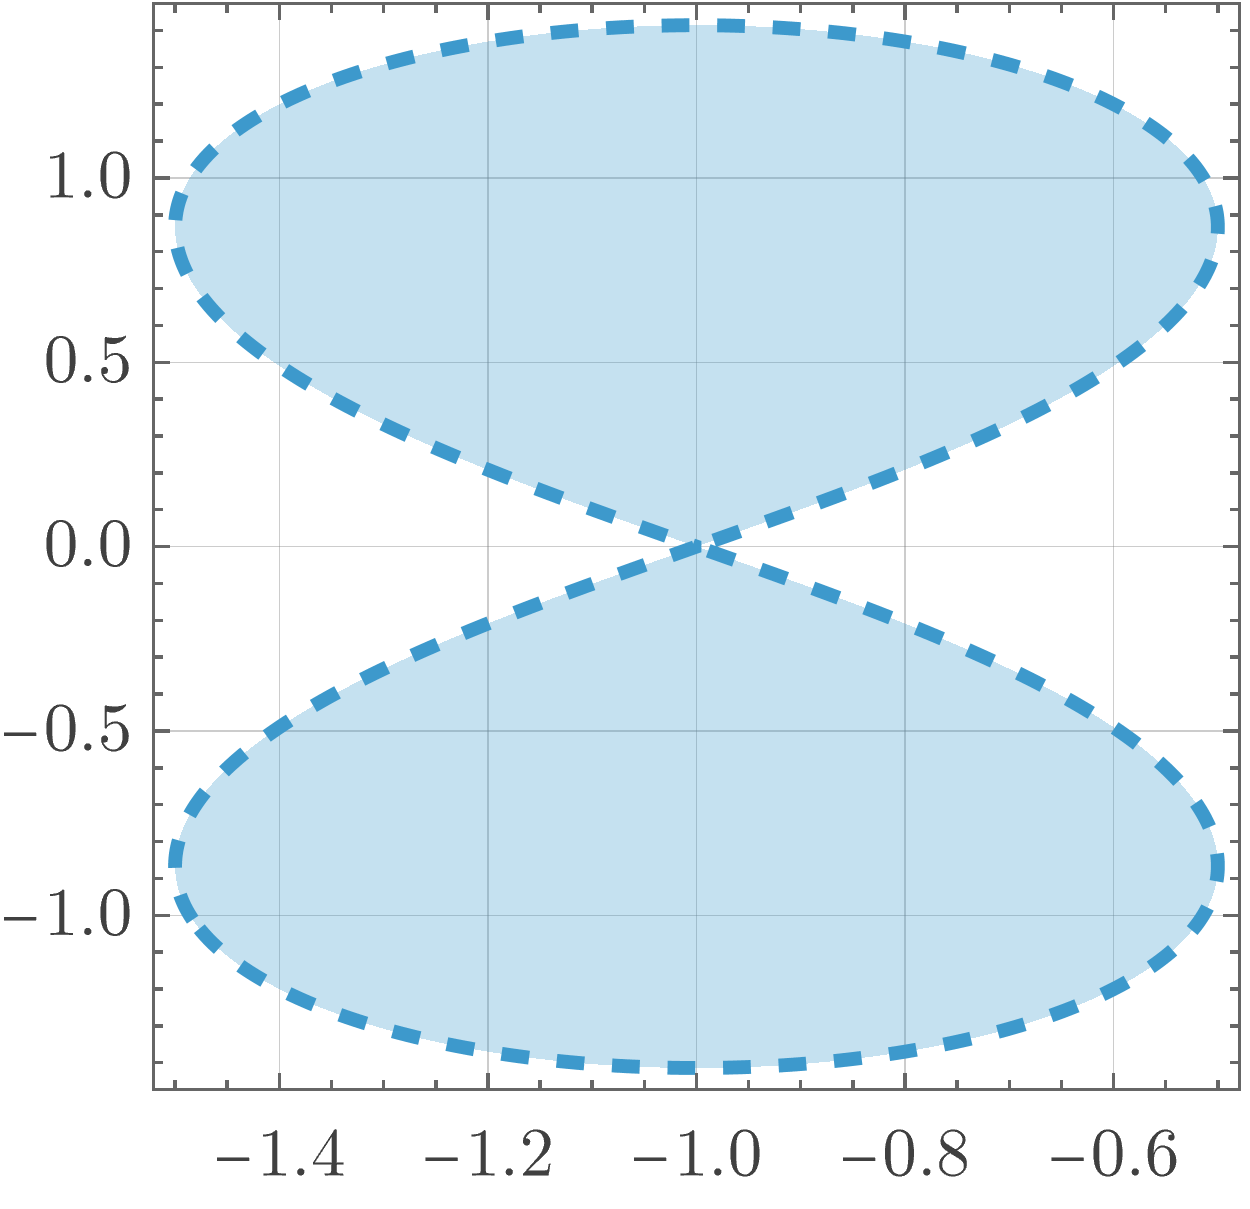
\includegraphics[width=0.4\linewidth]{figures/第7次作业-fig01.png}
    \end{center}
  \item
    令 \(a_n(z) = 2^n \sin(z/3^n)\)。

    我们用 d'Alembert 判别法 \(L = \displaystyle\lim_{n\to\infty} \Bigl|\frac{a_{n+1}(z)}{a_n(z)}\Bigr|\)

    \[
    L = \lim_{n\to\infty} \Bigl|\frac{2^{n+1}\sin(z/3^{n+1})}{2^n\sin(z/3^n)}\Bigr| = \lim_{n\to\infty} 2\Bigl|\frac{\sin(z/3^{n+1})}{\sin(z/3^n)}\Bigr|
    \]

    令 \(w_n = z/3^n\)，则 \(z/3^{n+1}=w_n/3\)。当 \(n\to\infty\) 时 \(w_n\to0\)。

    \[
    L = \lim_{w_n\to0} 2\Bigl|\frac{\sin(w_n/3)}{\sin(w_n)}\Bigr| = \lim_{w_n\to0} 2\Bigl|\frac{w_n/3}{w_n}\Bigr| = \frac23
    \]

    由于 \(L = 2/3 < 1\)，级数对所有 \(z\) 绝对收敛。

    收敛域为：\(\mathbb{C}\) (整个复平面)。
  \item
    令 \(a_n(z) = \dfrac{z^n}{1+z^{2n}}\)。

    \begin{enumerate}
      \item 当 \(|z| < 1\) 时：
        \[
        |a_n(z)| = \frac{|z|^n}{|1+z^{2n}|}
        \]
        \(\displaystyle\lim_{n\to\infty} |z|^{2n} = 0\)，故 \(\displaystyle\lim_{n\to\infty} |1+z^{2n}| = 1\)。
        级数 \(\sum |a_n(z)|\) 与几何级数 \(\sum |z|^n\) (收敛) 具有相同的收敛性 (由极限比较判别法)。
        故在 \(|z| < 1\) 时绝对收敛。

      \item 当 \(|z| > 1\) 时：
        \[
        a_n(z) = \frac{z^n}{z^{2n}(1+z^{-2n})} = \frac{(1/z)^n}{1+(1/z)^{2n}}
        \]
        令 \(w = 1/z\)，则 \(|w| < 1\)。
        \[
        a_n(z) = \frac{w^n}{1+w^{2n}}
        \]
        根据上一种情况，级数 \(\sum a_n(z)\) 绝对收敛。

      \item 当 \(|z| = 1\) 时：
        \[
        a_n(z) = \frac{z^n}{1+z^{2n}},\quad |a_n(z)| = \frac1{|1+z^{2n}|} \ge \frac1{1+|z|^{2n}} = \frac12
        \]
        故级数在 \(|z|=1\) 上发散。
    \end{enumerate}

    收敛域为：\(|z| < 1\) 或 \(|z| > 1\)，即 \(\mathbb{C}\setminus\{z: |z|=1\}\)。
\end{enumerate}
\end{solution}
\end{question}

\begin{question}
试求下列幂级数的收敛半径：
\begin{enumerate}
  \item \(\displaystyle\sum_{n=1}^{\infty} n^p z^n\)
  \item \(\displaystyle\sum_{n=1}^{\infty} q^{n^2} z^n\) 其中 \(|q| < 1\)
  \item \(\displaystyle\sum_{n=1}^{\infty} \frac{n!}{n^n} z^n\)
  \item \(\displaystyle\sum_{n=1}^{\infty} \frac{(-1)^n}{9^{2n}(n!)^2} z^n\)
  \item \(\displaystyle\sum_{n=1}^{\infty} n! \, z^n\)
  \item \(\displaystyle\sum_{n=1}^{\infty} \frac{z^n}{n!}\)
  \item \(\displaystyle\sum_{n=1}^{\infty} \frac{\ln n}{n!} z^n\)
  \item \(\displaystyle\sum_{n=1}^{\infty} \Bigl(1-\frac1n\Bigr)^{n} z^n\)
\end{enumerate}

\begin{solution}
\begin{enumerate}
  \item\(c_n = n^p\)。
    \[
    R = \lim_{n\to\infty} \Bigl|\frac{c_n}{c_{n+1}}\Bigr| = \lim_{n\to\infty} \frac{n^p}{(n+1)^p} = \lim_{n\to\infty} \Bigl(\frac{n}{n+1}\Bigr)^p = 1^p = 1
    \]
    \(R=1\)。
  \item\(c_n = q^{n^2}\)。
    \[
    \frac1R = \varlimsup_{n\to\infty} |c_n|^{1/n} = \varlimsup_{n\to\infty} (|q|^{n^2})^{1/n} = \varlimsup_{n\to\infty} |q|^n
    \]
    因为 \(|q| < 1\)，\(\displaystyle\lim_{n\to\infty} |q|^n = 0\)。
    \[
    1/R = 0 \Rightarrow R = \infty
    \]
    \(R = \infty\)。
  \item\(c_n = \dfrac{n!}{n^n}\)。
    \[
    R = \lim_{n\to\infty} \Bigl|\frac{c_n}{c_{n+1}}\Bigr| = \lim_{n\to\infty} \frac{n!}{n^n} \Big/ \frac{(n+1)!}{(n+1)^{n+1}}
    \]
    \[
    R = \lim_{n\to\infty} \frac{n!}{n^n} \cdot \frac{(n+1)^{n+1}}{(n+1)!} = \lim_{n\to\infty} \frac{n!(n+1)(n+1)^n}{n^n (n+1)n!} = \lim_{n\to\infty} \Bigl(\frac{n+1}{n}\Bigr)^n = \lim_{n\to\infty} \Bigl(1+\frac1n\Bigr)^n = \ee
    \]
    \(R = \ee\)。
  \item\(c_n = \dfrac{(-1)^n}{9^{2n}(n!)^2}\)。
    \[
    R = \lim_{n\to\infty} \Bigl|\frac{c_n}{c_{n+1}}\Bigr| = \lim_{n\to\infty} \frac{1}{9^{2n}(n!)^2} \Big/ \frac{1}{9^{2(n+1)}((n+1)!)^2}
    \]
    \[
    R = \lim_{n\to\infty} \frac{9^{2n+2}((n+1)!)^2}{9^{2n}(n!)^2} = \lim_{n\to\infty} \frac{9^2 (n+1)^2 (n!)^2}{(n!)^2} = \lim_{n\to\infty} 81(n+1)^2 = \infty
    \]
    \(R = \infty\)。
  \item\(c_n = n!\)。
    \[
    R = \lim_{n\to\infty} \Bigl|\frac{c_n}{c_{n+1}}\Bigr| = \lim_{n\to\infty} \frac{n!}{(n+1)!} = \lim_{n\to\infty} \frac1{n+1} = 0
    \]
    \(R = 0\)。
  \item\(c_n = \dfrac1{n!}\)。
    \[
    R = \lim_{n\to\infty} \Bigl|\frac{c_n}{c_{n+1}}\Bigr| = \lim_{n\to\infty} \frac{1/n!}{1/(n+1)!} = \lim_{n\to\infty} \frac{(n+1)!}{n!} = \lim_{n\to\infty} (n+1) = \infty
    \]
    \(R = \infty\)。
  \item\(c_n = \dfrac{\ln n}{n!}\)。
    \[
    R = \lim_{n\to\infty} \Bigl|\frac{c_n}{c_{n+1}}\Bigr| = \lim_{n\to\infty} \frac{\ln n}{n!} \Big/ \frac{\ln(n+1)}{(n+1)!}
    \]
    \[
    R = \lim_{n\to\infty} \frac{\ln n}{\ln(n+1)} \cdot \frac{(n+1)!}{n!} = \lim_{n\to\infty} \frac{\ln n}{\ln(n+1)} \cdot (n+1)
    \]
    由于 \(\displaystyle\lim_{n\to\infty} \frac{\ln n}{\ln(n+1)} = 1\) (由 L'H\^{o}pital 法则)，
    \[
    R = \lim_{n\to\infty} 1\cdot (n+1) = \infty
    \]
    \(R = \infty\)。
  \item 令 \(c_n=\Bigl(1-\dfrac1n\Bigr)^n\)。由 Cauchy--Hadamard 公式，
    \[
    \frac1R
    =\varlimsup_{n\to\infty}|c_n|^{1/n}
    =\lim_{n\to\infty}\left(1-\frac1n\right)
    =1.
    \]
    因而 \(R=1\)。
\end{enumerate}
\end{solution}
\end{question}

\begin{question}
证明级数 \(\displaystyle S(z) = \sum_{n=0}^{\infty} \Bigl(\frac{z^{n+1}}{n+1} - \frac{2z^{2n+3}}{2n+3}\Bigr)\) 的和函数在 \(z=1\) 点不连续，这与 Abel 第二定理矛盾吗？

\begin{solution}
在收敛域 \(|z|<1\) 内，我们可以将级数拆开并重排：

\[
S(z) = \sum_{n=0}^{\infty} \frac{z^{n+1}}{n+1} - \sum_{n=0}^{\infty} \frac{2z^{2n+3}}{2n+3}
\]

\[
S(z) = \sum_{k=1}^{\infty} \frac{z^{k}}{k} - \sum_{m=0}^{\infty} \frac{2z^{2m+3}}{2m+3}
\]

\[
S(z) = \Bigl(z + \frac{z^2}{2} + \frac{z^3}{3} + \frac{z^4}{4} + \frac{z^5}{5} + \cdots\Bigr) - 2\Bigl(\frac{z^3}{3} + \frac{z^5}{5} + \frac{z^7}{7} + \cdots\Bigr)
\]

\[
S(z) = z + \frac{z^2}{2} - \frac{z^3}{3} + \frac{z^4}{4} - \frac{z^5}{5} + \frac{z^6}{6} + \cdots
\]

\[
S(z) = 2z + \sum_{k=1}^{\infty} \frac{(-z)^k}{k} = 2z - \ln(1+z)
\]

因此和函数在 \(z=1^-\) 的极限为，\(\displaystyle\lim_{z\to 1^{-}} S(z) = 2 - \ln 2\)

当 \(z=1\) 时，有
\[
\begin{aligned}
S(1) &= \sum_{n=0}^{\infty} \Bigl(\frac1{n+1} - \frac{2}{2n+3}\Bigr) = \sum_{n=0}^{\infty} \Bigl(\frac{2}{2n+2} - \frac{2}{2n+3}\Bigr) \\
&= 2\Bigl(\frac12 - \frac13 + \frac14 - \frac15 + \cdots\Bigr) = 2 - 2\ln 2
\end{aligned}
\]

Abel 第二定理指出：若幂级数 \(\displaystyle\sum_{n=0}^{\infty} c_n z^n\) 在 \(z=1\) 处收敛，则 \(\displaystyle\lim_{z\to 1^{-}} \Bigl(\sum_{n=0}^{\infty} c_n z^n\Bigr) = \sum_{n=0}^{\infty} c_n\)。但题给的 \(S(z)\) 在 \(|z|>1\) 发散，因此无法将其重新分组，变为幂级数，违反了 Abel 第二定理的前提条件。
\end{solution}
\end{question}

\begin{question}
将下列函数在指定点展开为 Taylor 级数，并给出其收敛半径：
\begin{enumerate}
  \item \(\displaystyle\frac1{1+z+z^2}\)，在 \(z=0\) 展开
  \item \(\sin z\)，在 \(z=n\pi\) 展开，\(n=0,\pm1,\pm2,\dots\)
  \item \(\displaystyle\frac1{(1-z)^m}\)，其中 \(m\) 为正整数，在 \(z=0\) 展开
\end{enumerate}

\begin{solution}
\begin{enumerate}
  \item
    \(f(z)=\dfrac1{1+z+z^2}=\dfrac{1-z}{(1-z)(1+z+z^2)}=\dfrac{1-z}{1-z^3}\).

    对于 \(|z^3|<1\) (即 \(|z|<1\))：

    \[
    f(z)=(1-z)\sum_{n=0}^{\infty} (z^3)^n = (1-z)\sum_{n=0}^{\infty} z^{3n}
    \]

    \[
    f(z)=\sum_{n=0}^{\infty} z^{3n} - \sum_{n=0}^{\infty} z^{3n+1}
    \]

    \textbf{Taylor 级数}：\(\displaystyle\sum_{n=0}^{\infty} (z^{3n} - z^{3n+1})\).

    \textbf{收敛半径}：函数的奇点是 \(1+z+z^2=0\) 的根，即 \(z=\ee^{\pm\ii 2\pi/3}\)。
    奇点到 \(z=0\) 的最近距离为 \(|\ee^{\pm\ii 2\pi/3}|=1\)。
    收敛半径 \(R=1\)。
  \item
    令 \(w=z-n\pi\)，则有 \(\sin z = (-1)^n\sin w\).

    将 \(\sin w\) 在 \(w=0\) 处展开：

    \[
    \sin z = (-1)^n \sum_{m=0}^{\infty} \frac{(-1)^m}{(2m+1)!} w^{2m+1}
    \]

    \[
    \sin z = \sum_{m=0}^{\infty} \frac{(-1)^{n+m}}{(2m+1)!} (z-n\pi)^{2m+1}
    \]

    \textbf{Taylor 级数}：\(\displaystyle\sum_{m=0}^{\infty} \frac{(-1)^{n+m}}{(2m+1)!} (z-n\pi)^{2m+1}\).

    \textbf{收敛半径}：\(\sin z\) 是整函数，在 \(\mathbb{C}\) 上解析，故收敛半径 \(R=\infty\)。
  \item
    我们知道 \(\displaystyle\frac1{1-z}=\sum_{n=0}^{\infty} z^n\).

    将此式对 \(z\) 求导 \(m-1\) 次：

    \[
    \dv{}{z}\Bigl(\frac1{1-z}\Bigr) = (1-z)^{-2}
    \]

    \[
    \dv{^2}{z^2}\Bigl(\frac1{1-z}\Bigr) = 2(1-z)^{-3}
    \]

    \[
    \frac{d^{m-1}}{dz^{m-1}}\Bigl(\frac1{1-z}\Bigr) = (m-1)!\,(1-z)^{-m}
    \]

    因此，

    \[
    \begin{aligned}
    \frac1{(1-z)^m} &= \frac1{(m-1)!}\frac{d^{m-1}}{dz^{m-1}}\Bigl(\sum_{n=0}^{\infty} z^n\Bigr) \\
    &= \frac1{(m-1)!}\sum_{n=m-1}^{\infty} \frac{d^{m-1}}{dz^{m-1}}z^n \\
    &= \frac1{(m-1)!}\sum_{n=m-1}^{\infty} n(n-1)\cdots(n-m+2)\,z^{n-m+1} \\
    &= \frac1{(m-1)!}\sum_{n=m-1}^{\infty} \frac{n!}{(n-m+1)!}\,z^{n-m+1}
    \end{aligned}
    \]

    令 \(k=n-m+1\)，则 \(n=k+m-1\).

    \[
    \frac1{(1-z)^m} = \frac1{(m-1)!}\sum_{k=0}^{\infty} \frac{(k+m-1)!}{k!}z^k = \sum_{k=0}^{\infty} \binom{k+m-1}{k} z^k
    \]

    \textbf{Taylor 级数} (用 \(n\) 作指标)：\(\displaystyle\sum_{n=0}^{\infty} \binom{n+m-1}{n} z^n\).

    \textbf{收敛半径}：函数 \(f(z)=(1-z)^{-m}\) 唯一的奇点在 \(z=1\)。奇点到 \(z=0\) 的距离为 1。收敛半径 \(R=1\)。
\end{enumerate}
\end{solution}
\end{question}
